\chapter{Interfaces between hydrodynamics and transport} \label{ch:interfaces}

As one can see from the discussion about hydrodynamical and hybrid models, many
uncertainties in the dynamical simulations of heavy ion collision are coming from
interfaces between different approaches - for hybrid models this is the construction of
the initial state (fluidization) and final state (particlization). In this chapter the
actual calculations at these interfaces are discussed to better understand the source
of uncertainties and to introduce the methodology used in the next chapters.
Some parts of this chapter follow publications \cite{Oliinychenko:2014tqa},
\cite{Oliinychenko:2015lva} and \cite{Oliinychenko:2016vkg}.

\section{Coarse-graining} \label{sec:coarse_graining}

\begin{sidewaysfigure}
  \centering
  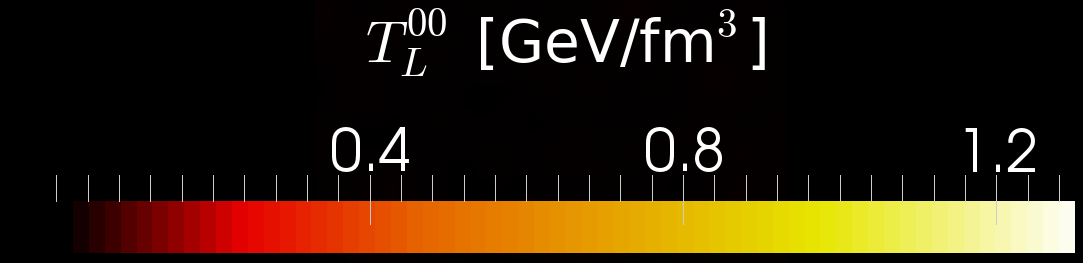
\includegraphics[width = 0.3\textwidth]{illustrations/coarse_graining/color_legend_T00.png} \\
  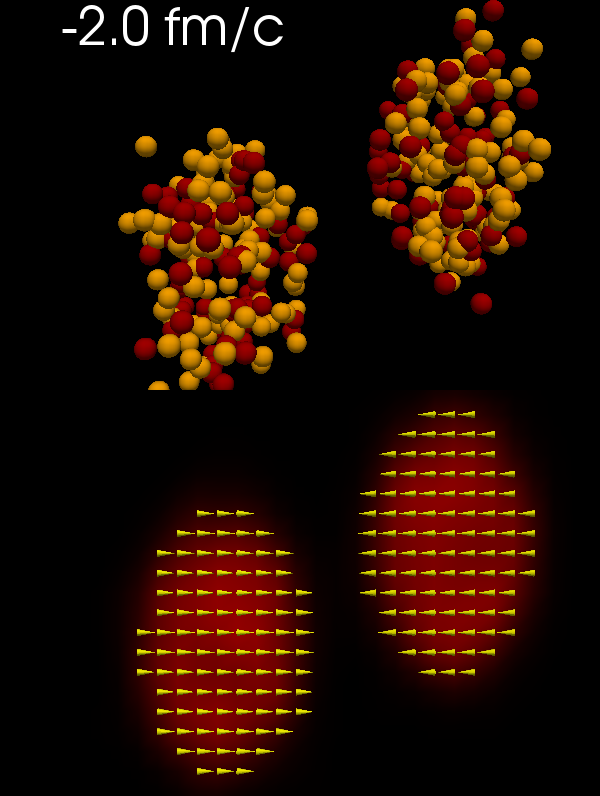
\includegraphics[width = 0.32\textwidth]{illustrations/coarse_graining/coarse_AuAu_sqrts3GeV_b5_0000.png}
  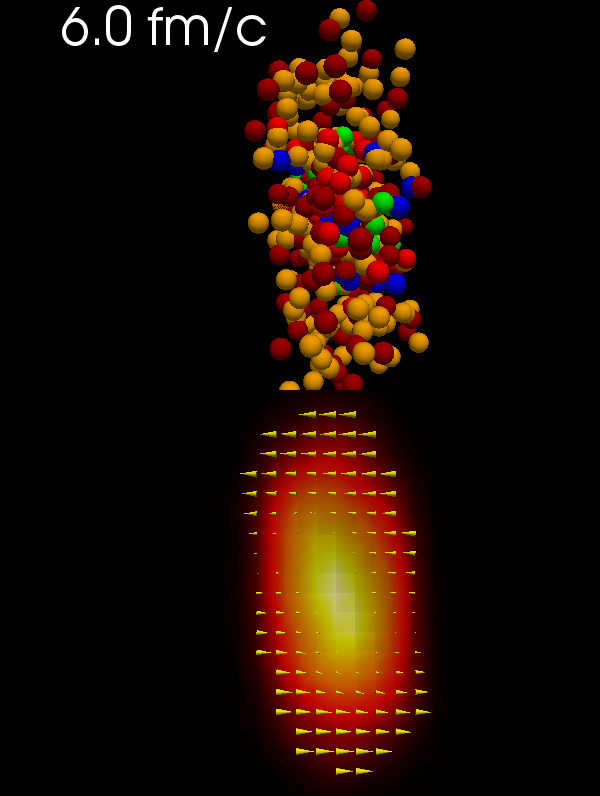
\includegraphics[width = 0.32\textwidth]{illustrations/coarse_graining/coarse_AuAu_sqrts3GeV_b5_0004.png}
  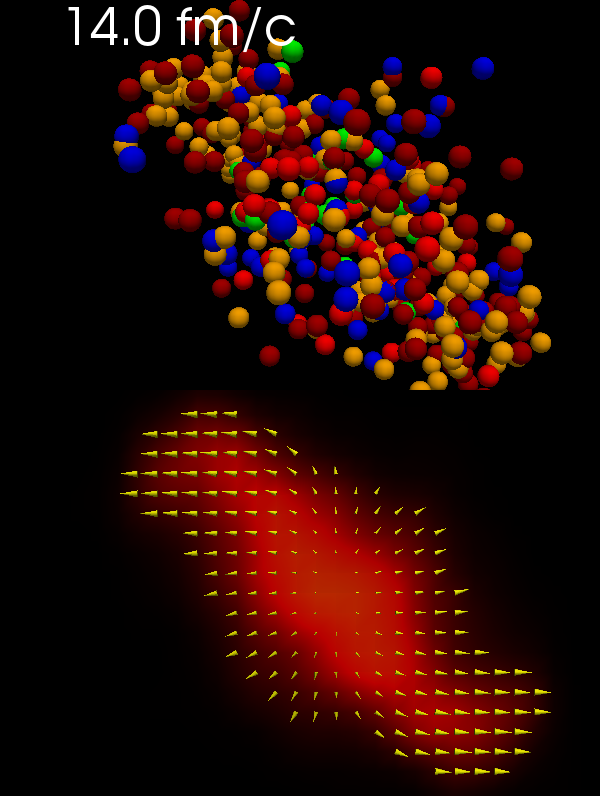
\includegraphics[width = 0.32\textwidth]{illustrations/coarse_graining/coarse_AuAu_sqrts3GeV_b5_0008.png}
  \caption{Demonstration of coarse-graining. On the top row is the particle
           representation of a Au+Au
           collision at $\sqrt{s} = $ 3 GeV and impact parameter $b = $
           5 fm from the transport code SMASH. The simulation was performed in the
           center of mass frame, that is why both nuclei are Lorentz-contracted.
           Dark-red corresponds to protons,
           yellow to neutrons, blue to pions, red to $\Delta$s and green to the rest.
           At the bottom is the coarse-grained picture of the energy-density in the
           Landau rest
           frame and Landau velocities in the XZ plane from a SMASH simulation with
           $N_{test} = 30$.}
  \label{fig:HIC_exp_mindmap}
\end{sidewaysfigure}

Coarse-graining is a method to obtain macroscopic variables, such as
the rest-frame energy-density, baryon density or velocity of the fluid from
the particles in a transport approach. This method is used extensively in chapters
\ref{chap:local_equilibration}, \ref{chap:cooper_frye} and \ref{chap:forced_therm}, as
well as in other works, e.g. \cite{Huovinen:2002im,Endres:2014zua}.
An example of coarse-graining is demonstrated in Fig. \ref{fig:HIC_exp_mindmap},
where the microscopic particles from a transport simulation of heavy ion collision are
turned into energy-density, pressure and velocity, the macroscopic variables necessary
for hydrodynamics.

In the following sections the mathematical expressions for coarse-graining are derived,
starting from the energy-momentum tensor and four-currents for a point-like particle,
and proceeding with a smeared particle or a wavepacket.

\subsection{Energy-momentum tensor of a point-like particle}

The expression for the energy-momentum tensor of a single point-like particle is
well-known in the literature \cite{LL_ED}, as well as for particles interacting
with fields \cite{Sutherland:2015}. Here the derivation is repeated to use it
later for the wavepacket.

The action of a point-like particle is

\begin{equation}
  S = -m \int_a^b d\tau = -m \int_a^b \sqrt{dx^{\mu}dx_{\mu}} \,.
\end{equation}

Varying the particle trajectory $x^{\mu} = x^{\mu} + \delta x^{\mu}$ with
fixed ends one obtains an action variation:

\begin{align}
  \delta S = -m \int_a^b \sqrt{dx^{\mu}dx_{\mu} + 2 dx^{\mu} d\delta x_{\mu}} +
             m \int_a^b \sqrt{dx^{\mu}dx_{\mu}} = \nonumber \\
             = -m \int_a^b \frac{dx^{\mu}}{d\tau} d\delta x_{\mu} = \nonumber \\
             = m \int_a^b \frac{du^{\mu}}{d\tau} d\tau \delta x_{\mu} \,,
\end{align}

where $u^{\mu} = \frac{dx^{\mu}}{d\tau}$. Using the expression

\begin{equation}
  \frac{du^{\mu}}{d\tau} = \frac{\partial u^{\mu}}{\partial x^{\nu}} \frac{\partial x^{\nu}}{\partial \tau}
   = u^{\nu} \partial_{\nu} u^{\mu}
\end{equation}

one can rewrite the action variation as

\begin{equation}
  \delta S = m \int_a^b u^{\nu} \partial_{\nu} u^{\mu} d\tau \delta x_{\mu} \,.
\end{equation}

In this expression variation of the action depends on the coordinates and velocity
of the particle, that will further be marked with index ``p''. Now let us rewrite
it in terms of continuous medium by adding integration over space-time and a $\delta$-function. The coordinates $x^{\mu}$ are coordinates in
space, over which integration is performed.

\begin{equation} \label{eq:ds}
  \delta S = m \int dV \int_a^b d\tau \delta^{(4)}(x^{\mu} - x^{\mu}_p(\tau)) u^{\nu} \partial_{\nu} u^{\mu} \delta x_{\mu} \,.
\end{equation}

The delta-function $\delta^{(4)}(x^{\mu} - x^{\mu}_p(\tau))$ allows to change
variables depending on $x^{\mu}_p$ to variables dependent on $x^{\mu}$. Since
$\int d\tau \delta(x^{0} - x^{0}_p(\tau)) = \frac{1}{u^{0}}$,
one can rewrite the equation (\ref{eq:ds}) in the following form:

\begin{align}
  \delta S = \int dV \, \partial_{\nu} \Tmn \delta x_{\mu}   \,,
\end{align}

where the following notation is used

\begin{align}
  \Tmn = m \jmu u^{\nu} \,, \\
  \jmu = u^{\mu} \delta^{(4)}(x^{\mu} - x^{\mu}_p(\tau)) = \frac{u^{\mu}}{u^{0}} \delta^{(3)}(x^{i} - x^{i}_p(\tau)) \,.
\end{align}

Here it was taken into account that $\partial_{\mu} \jmu = 0$ due to the
equations of motion. It is convenient to rewrite this in terms of the
4-momentum $p^{\mu}$ of the particle:

\begin{align} \label{eq:tmn_pointlike}
  \jmu = \frac{p^{\mu}}{p^0} \delta^{(3)}(x^i - x^i_p(\tau)) \\
  \Tmn = \frac{p^{\mu}p^{\nu}}{p^0} \delta^{(3)}(x^i - x^i_p(\tau))
\end{align}

There is a simpler way to obtain the same formulas. One notices from the
 $\Tmn$ of the ideal fluid that for a particle at rest

\begin{equation}
  \Tmn_{\mathrm{rest}}(\vec{x}) = \mathrm{diag}(m \delta^{(3)}(x^i - x^i_p), 0, 0, 0)
\end{equation}

Notice that the $\delta$-function has dimension of fm$^{-3}$ here. Boosting the
energy-momentum tensor with the 4-velocity $u^{\mu}$ using the Lorentz boost matrices
from Eq. (\ref{eq:lorentz_boost_matr}) one obtains

\begin{equation}
  \Tmn(\vec{x}') = \Lambda^{\mu}_0 \Lambda^{\nu}_0 m \delta^{(3)}(x'^i - x'^i_p)
                   \frac{1}{u^0}
           = \frac{p^{\mu}p^{\nu}}{p^0} \delta^{(3)}(x'^i - x'^i_p) \,.
\end{equation}

Note that the necessary $\frac{1}{u^0}$ factor is obtained via the $\delta$-function transformation:

\begin{align}
  d^3x \delta^{(3)}(x^i - x^i_p) = d^3x' \delta^{(3)}(x'^i - x'^i_p) \,, \\
  d^3x  = u^0 d^3x' \,.
\end{align}

The primed coordinates $x'$ here are the lab frame coordinates in contrast to
the ones in the rest frame. For $\jmu$ the calculation is analogous.

\subsection{Energy-momentum tensor of a wavepacket} \label{sec:tmn_wavepacket}

As one can see from Eq. (\ref{eq:tmn_pointlike}), for finite numbers of point-like
particles  the energy-momentum tensor will be non-zero only at the particle
positions. For coarse-graining it is desirable that $\Tmn$ is continuous in
space. That is why the point-like particles are not used directly. Instead they
are smeared, which may be physically interpreted as wavepackets in coordinate space.

To introduce a non-pointlike particle one simply replaces the $\delta$-function in
space by a smearing kernel $K(\vec{x} - \vec{x}_p, u^{\mu}_p, \sigma)$, which
represents the shape of the wavepacket in the rest frame. The smearing kernel should
satisfy three conditions: $K(\vec{r})d^3r$ should be Lorentz scalar, it should be
normalized as $\int K(\vec{x} - \vec{x}_p) d^3x = 1$, and it should approach a
$\delta$-function when the smearing parameter $\sigma$ approaches zero. Then
transforming from the particle rest frame

\begin{align}
  \Tmn_{\mathrm{rest}}(\vec{x}) = \mathrm{diag}(m K(\vec{x} - \vec{x}_p), 0, 0, 0) \\
  \jmu_{\mathrm{rest}}(\vec{x}) = \mathrm{diag}(K(\vec{x} - \vec{x}_p), 0, 0, 0)
\end{align}

exactly as it was done with the $\delta$-function, one obtains:

\begin{align} \label{eq:one_part_tmn}
  \jmu(\vec{x}') = \frac{p^{\mu}}{p^0} K(\vec{x}' - \vec{x}'_p(\tau)) \\
  \Tmn(\vec{x}') = \frac{p^{\mu}p^{\nu}}{p^0} K(\vec{x}' - \vec{x}'_p(\tau)) \,.
\end{align}

Surprisingly, all current popular choices of $K$ in the literature are such that
$K(\vec{r})d^3r$ is not a Lorentz scalar:

\begin{itemize} %[noitemsep]
  \item Cell averaging: $K(\vec{x}) = \begin{cases} 1/\Delta V, \, \vec{x} \in \Delta V \\
                                                  0, \text{otherwise} \end{cases}$.
        Here $K(\vec{x})d^3x$ is not a Lorentz scalar,
        since the volume $\Delta V$ is not contracted.
  \item Gaussian distribution with Lorentz contraction in z direction:
        $K(\vec{x}) = N exp\left(-\frac{x^2 + y^2 + \gamma_z^2 z^2}{2 \sigma^2} \right)$
        is behaving properly only under boosts in z direction.
  \item Gaussian in $x$, $y$, $\eta$ coordinates also behaves
        properly only under boosts in z direction.
\end{itemize}

Let us derive a simple, not too computationally demanding kernel, which
satisfies all aforementioned conditions, in particular $K(\vec{x} - \vec{x}_p)d^3x$
being a Lorentz scalar. In the rest frame of the particle a Gaussian is taken, assuming
that the particle is at the origin, $\vec{x}_p = 0$:

\begin{equation}
  K_{rf}(\vec{x}) = (2\pi \sigma^2)^{-3/2} exp(-\vec{x}^2/2\sigma^2)
\end{equation}

Let us now express the rest frame coordinates through coordinates $\vec{x}'$ in the
laboratory (computational) frame via the Lorentz boost using the matrix from
Eq. (\ref{eq:lorentz_boost_matr}).

\begin{align}
  \left( \begin{array}{c}  t \\ x^i \end{array} \right)
  = \left( \begin{array}{cc}
           u^0  &  u^i  \\
           u^i  &  \delta^{ij} + (1+u^0)^{-1} u^i u^j
    \end{array} \right)
  \left( \begin{array}{c}  0 \\ x'^j \end{array} \right)
\end{align}

The time component on the right hand side is zero because the smearing kernel
needs to be evaluated at a fixed time in the computational frame,
not in the particle rest frame. This derivation is analogous to the
standard derivation of the Lorentz contraction, but the direction of contraction
is not necessarily along a coordinate axis.

It follows then that

\begin{align}
  x^i = (\delta^{ij} + (1+u^0)^{-1} u^i u^j) x'^j = x'^i + (1+u^0)^{-1} u^i (u^j x'^j) \\
  \vec{x}^2 = x^i x^i = \vec{x}'^2 + 2 (1+u^0)^{-1} (u^i x'^i) (u^j x'^j) + (1+u^0)^{-2} (u^i u^i) (u^j x'^j)^2 = \\
  = \vec{x}'^2 + (u^j x'^j)^2 (1+u^0)^{-1} \parenths{2 + \frac{(u^i u^i)}{1+u^0}}
\end{align}

It follows from  $u^{\mu} u_{\mu} = 1$ that $u^i u^i = u_0^2 - 1$ and

\begin{equation}
  (1+u^0)^{-1} \parenths{2 + \frac{(u^i u^i)}{1+u^0}} = 1 \,.
\end{equation}

Therefore,

\begin{equation}
  \vec{x}^2 = \vec{x}'^2 + (u^j x'^j)^2
\end{equation}

and the kernel $K$ can be written in the computational frame as

\begin{equation} \label{eq:smearing_kernel}
  K(\vec{x}' - \vec{x}'_p, u_p, \sigma) = \frac{u_0}{(2\pi \sigma^2)^{3/2}}
  \expOf{-\frac{\vec{x}'^2 + (\vec{u} \vec{x}')^2}{2\sigma^2}}
\end{equation}

This is the kernel used for all calculations throughout this thesis.
The factor $u_0$ was added to ensure  $ K(x' - x'_p) d^3x' = K_{rest}(x - x_p)
d^3x_{rest}$, since $d^3x' = u_0^{-1} d^3x_{rest}$. Let us check explicitly
that the normalization condition is fulfilled. Using the Gaussian integral

\begin{equation}
  \int \left( \prod_{i=1}^{n} dx_i \right) e^{-x_i A^{ij} x_j}  = \pi^{n/2} \, (det A)^{-1/2}
\end{equation}

and the fact that the determinant $det(\delta_{ij} + u_i u_j) = u_0^2$ one
indeed finds that

\begin{equation}
  \int K(\vec{x}' - \vec{x}'_p) d^3x' = 1 \,.
\end{equation}

It is not a coincidence that the smearing kernel is correctly normalized.
It already follows from the transformation properties, that if it is
normalized in one frame, it is normalized in any frame. One can check that this
formula turns into the more familiar expression from \cite{Huovinen:2012is}, if
the particle velocity is directed along the z-axis and $\vec{u} = \gamma_z(0, 0,
\beta_z)$. Since $1 + (\gamma_z \beta_z)^2 = \gamma_z^2$, it follows that
$\vec{x}'^2 + (u^j x'^j)^2 = x'^2 + y'^2 + \gamma_z^2 z'^2$ and the coincidence
of the expressions is established.

The last thing to check is that the smearing kernel approaches the $\delta$-function
at $\sigma \to 0$. If this is true in the rest frame, it is true in any frame,
so is enough to check it at the rest frame. This can be immediately seen from
 the $\delta$-function limit representation

\begin{equation}
  \delta(x) = \lim_{\epsilon \to 0} \frac{1}{\sqrt{2 \pi \epsilon}} e^{- \frac{x^2}{2\epsilon}} \,.
\end{equation}

Taking this limit for every dimension one obtains

\begin{equation}
  \lim_{\sigma \to 0} K_{rest}(\vec{x} - \vec{x}_p, \sigma) =
  \delta^{(3)}(\vec{x} - \vec{x}_p) \,.
\end{equation}

Finally one notes that the exponential form of the smearing function is by no
means unique. Any normalized function of $\vec{x}'^2 + (u^j x'_j)^2$ can be
incorporated given that in some limit it gives the $\delta$-function. The reasons to
prefer an exponential are firstly, because it has infinite number of continuous
derivatives and secondly, because it corresponds to the physical background of the Gaussian wavepacket.  An alternative smearing kernel could be, for example,

\begin{equation}
  K_{\mathrm{alternative}} = \begin{cases}
    \frac{15 u_0}{8 \pi \sigma^3} \parenths{1 - \frac{\vec{x}'^2 + (\vec{u} \vec{x}')^2}{\sigma^2}} & |x| < \sigma \\
    0  & |x| > \sigma
 \end{cases}
\end{equation}

\subsection{Final expressions for coarse-graining} \label{sec:final_coarse_graining}

The derivations from the two previous sections allow to write down the expressions used
in this work for the coarse-graining. Suppose that particles for coarse-graining are
taken from $N_{ev}$ events ($N_{ev}$ transport simulations). Then the following
expressions are valid:

\begin{align}
  \Tmn(\vec{r}) = \frac{1}{N_{ev}} \sum_{events} \sum_i
                  \frac{p^{\mu}_i p^{\nu}_i}{p^0_i} K(\vec{r} - \vec{r_i}, u_i) \\
  \jmu(\vec{r}) = \frac{1}{N_{ev}} \sum_{events} \sum_i
                  \frac{p^{\mu}_i}{p^0_i} K(\vec{r} - \vec{r_i}, u_i) \\
  K(\vec{r} - \vec{r_i}, u, \sigma) = \frac{u_0}{(2\pi \sigma^2)^{3/2}}
                  \expOf{-\frac{(\vec{r} - \vec{r_i})^2 +
                                (\vec{u} \cdot (\vec{r} - \vec{r_i}))^2}{2\sigma^2}} \\
  u^{\mu} = (u^0, \vec{u}) = \frac{p^{\mu}}{m}
\end{align}

These expressions in principle allow to compute the energy-momentum tensor and
four-currents on any irregular grid, but in this work only Cartesian grids are used.

\section{Fluidization} \label{sec:fluidization}

The first interface in hybrid approaches is the transition from transport to fluid,
called fluidization. At fluidization microscopic particles with their coordinates and
momenta have to be converted into a macroscopic continuous hydrodynamic fields: density,
energy density, pressure, etc. In the relativistic case the first step of the
fluidization is the construction of the energy-momentum tensor $\Tmn$ and four-currents
$\jmu$ as describe above. However, it is by no means guaranteed that they have an ideal
fluid-dynamical form or that they are close to it. Indeed, transport
approaches generally simulate non-equilibrium systems and the $\Tmn$ of hydrodynamics
is close to equilibrium. The problem of matching a non-equilibrium $\Tmn$
to an equilibrium one is relevant for many approaches that construct their initial state
from the discrete degrees of freedom \cite{Petersen:2008dd,Skokov:2005ut,Werner:2010aa,
Andrade:2005tx,Gale:2012rq,Karpenko:2015xea,Pang:2012he,Bhalerao:2015iya}.

This matching problem can be eliminated or minimized by waiting until transport
approach reaches equilibrium and only switching to hydrodynamics, when the necessary
degree of equilibration is reached. However, it was argued that a good description of
experimental data requires rather small initialization times of hydrodynamics
($\tau \leq 0.6$ fm/c at the highest RHIC energy) \cite{Heinz:2004pj}. The initial state
generated by transport at this early time is highly off-equilibrium. Such an initial
state is suitable for anisotropic hydrodynamics \cite{Strickland:2014pga},
but in most of the existent approaches it has to be matched to equilibrium state.
The matching procedure is not unique and introduces uncertainty to the simulation. 
To demonstrate this uncertainty the matching procedures applied by different
approaches are discussed in section \ref{Sec_II}. All the discussed approaches
neglect the non-equilibrium part of $\Tmn$.

How good is this approximation? This depends on
the degree of thermalization at the time of fluidization. One way to quantify the
degree of thermalization is given in section \ref{Sec_III}. At high energies
a number of studies were devoted to understand the approach to equilibrium
in heavy ion collisions. It was studied both in strongly-coupled and weakly-coupled
field-theoretical models (see \cite{Strickland:2013uga} for an overview). The strongly
coupled ones apply dualities of supersymmetric Yang-Mills gauge theory for
calculations in the strong coupling limit \cite{Heller:2011ju,vanderSchee:2013pia}.
The weakly coupled ones are able to achieve fast thermalization in a weak coupling
limit, where colliding nuclei are described in the color-glass condensate framework
\cite{Gelis:2010nm,Lappi:2010ek}. The primary effect in CGC
leading to fast thermalization is believed to be plasma instabilities, such as
the chromo-Weibel instability~\cite{Arnold:2004ti}. Both types of approaches
predict considerable momentum space anisotropies at the time, when
hydrodynamics is initialized. The aforementioned studies are relevant for high
collision energies. At intermediate energies thermalization was studied using
transport models \cite{Bravina:2008ra}, where momentum distributions were
averaged over a ($5 \times 5 \times 5$) fm$^3$ central cell. This study
investigates global thermalization in a big volume and results in thermalization
times much larger than typical starting times for hydrodynamics. At the same
time, it is clear that thermalization is a local phenomenon. It is reached faster,
where the density is higher and collisions are more intense and probably never reached
at the boundary of the fireball. Therefore, in chapter \ref{chap:local_equilibration}
the deviation from equilibrium at intermediate energies is studied locally using
a coarse-grained transport approach.

\subsection{Overview of fluidization in current hybrid models} \label{Sec_II}

How do existing approaches perform fluidization, i.e. construct the initial state
of hydrodynamics? How is fluidization time chosen? What fluidization procedures
are applied (it was mentioned already that the procedure is not unique)? This is
discussed in this section.

The modern hybrid models applying fluidization are summarized in Table
\ref{Tab:models}. All the shown approaches need to obtain the ideal fluid part of
$\Tmn$ and $\jmu$ from discrete degrees of freedom (hadrons, partons, strings). The
viscous corrections are neglected in all models, even if viscous hydrodynamics is
applied for the evolution. The only exception is a recent work by Liu et
al.\cite{Liu:2015nwa}, where the initial stage for viscous hydrodynamics is
constructed from free streaming partons and viscous corrections are explicitly
included.

\begin{table*}
  \begin{tabular}{p{2.5cm}p{2.5cm}p{2.5cm}p{3cm}p{2.5cm}p{2.5cm}p{2.5cm}}
  \toprule[1.5pt]
   Model      &   Initial condition  & Hydro  & Switching \newline criterion &
   Smearing \newline kernel & Getting \newline $\Tmn_{ideal}$ \\

   \midrule[1pt]
     UrQMD \newline hybrid~\cite{Petersen:2008dd} &
     UrQMD \newline cascade &
     ideal 3+1D,\newline SHASTA &
     $t_{CM} \text{[fm/c]} =$ \newline $max(2R \sqrt{\frac{\Elab}{2m_N}}, 1.0)$ &
     Gaussian \newline z-contracted &
     $T^{\mu 0}$, $j^0$ \\

     Skokov-Toneev \newline hybrid~\cite{Skokov:2005ut} &
     Quark-Gluon- \newline String-Model &
     ideal 3+1D,\newline SHASTA &
     $t_{CM}$ such \newline that $S/Q_B = \text{const}$ &
     not \newline mentioned &
     $T^{\mu 0}$, $j^0$ \\

     EPOS~\cite{Werner:2010aa} &
     Strings (Regge-\newline Gribov model) &
     ideal 3+1D &
     $\tau$ &
     Gaussian \newline z-contracted &
     Landau frame \\

     NeXSPheRIO \newline hybrid~\cite{Andrade:2005tx,Drescher:2000ec} &
     Strings (Regge-\newline Gribov model) &
     ideal 3+1D, \newline SPH &
     $\tau = 1$ fm/c \cite{Hama:2004rr} &
     Gaussian in \newline $x$, $y$, $\tau \eta$&
     Landau frame \\

     Gale et al~\cite{Gale:2012rq} &
     IP-glasma &
     viscous 3+1D,\newline MUSIC &
     $\tau = 0.2$ fm/c \newline ($\sqrt{s_{NN}} = 2.76$ TeV) &
     not \newline mentioned &
     Landau frame \\

     Karpenko \newline hybrid~\cite{Karpenko:2015xea} &
     UrQMD \newline cascade &
     viscous 3+1D &
     $\tau_{geom}$ &
     Gaussian with \newline $\sigma_{\perp}$ and $\sigma_{\eta}$ &
     $T^{\mu 0}$, $j^0$ \\

     Pang et al \newline hybrid~\cite{Pang:2012he} &
     AMPT &
     ideal 3+1D, \newline SHASTA &
     $\tau$ &
     Gaussian with \newline $\sigma_{\perp}$ and $\sigma_{\eta}$ &
     $T^{\mu 0}$, $j^0$ \\

     Bhalerao et al \newline hybrid~\cite{Bhalerao:2015iya} &
     AMPT &
     viscous 2+1D, \newline VISH2+1 &
     $\tau = 0.4$ fm/c \newline ($\sqrt{s_{NN}} = 2.76$ TeV) &
     Gaussian in \newline $x$, $y$ &
     local CM frame \\

  \bottomrule[1.5pt]
  \end{tabular}
  \caption{Fluidization features in different hybrid approaches. Each of these
           models, including those using viscous hydrodynamics, neglects viscous
           corrections at fluidization.}
  \label{Tab:models}
\end{table*}

In the relevant approaches \cite{Petersen:2008dd,Skokov:2005ut,Werner:2010aa,
Andrade:2005tx,Gale:2012rq,Karpenko:2015xea,Pang:2012he,Bhalerao:2015iya} the
fluidization is typically performed either at a constant proper time hypersurface
$\tau = const$ or at a constant center of mass frame time hypersurface $t_{CM} =
const$, see Table \ref{Tab:models}. The constant is often chosen according to the
\emph{geometrical criterion} - the time, when nuclei geometrically pass through each
other: $t_{CM} = \frac{2R}{\gamma \beta} = 2R (\Elab/2m_N)^{-1/2}$, where $R$ is
the radius of the nucleus, $\vec{\beta}$ is the velocity, $\gamma = (1 -
\vec{\beta}^2)^{-1/2}$, $\Elab$ is laboratory frame kinetic energy per nucleon, and
$m_N$ is nucleon mass. This time is taken to be the same for all collision
centralities. It was never systematically verified, if the energy-momentum tensor $\Tmn$
and four-currents $\jmu$ are close to hydrodynamical form at fluidization. An
exception is the work \cite{Skokov:2006us}, where the fluidization time $t_{fl}$ is
chosen such that the entropy per baryon does not change any more at $t > t_{fl}$. The
isochronous fluidization has little physical motivation, it is rather a matter of
technical convenience. Indeed, a study has appeared recently, where fluidization is not isochronous \cite{Shen:2017ruz}.

There are three ways in the literature to match the $\Tmn$ and $\jmu$
to ideal hydrodynamics. The first one is to use only $T^{\mu0}$, $j^0$, assuming
that they have ideal fluid form $\Tmn_{ideal} = (\epsilon + p)u^{\mu}u^{\nu} - p
g^{\mu \nu}$, $\jmu_{ideal} = n u^{\mu}$, and adding the equation of state
$p = p(\epsilon,n)$. The following system of equations is then solved (usually
iteratively, for details see \cite{Pang:2012he}):

\begin{align} \label{eq:rest_frame_cons}
  \begin{cases}
    T^{00} = (\epsilon + p) \gamma^2 - p \\
    T^{0i} = (\epsilon + p) \gamma^2 \vec{v} \\
    j_B^0 = n \gamma \\
    p = p_{EoS}(n, \epsilon)
  \end{cases}
\end{align}

The advantage of this method is that it conserves energy and momentum. However,
this method supports switching only to ideal fluid $\Tmn_{ideal}$, keeping
viscous corrections is hardly possible. Even though the switching method
conserves energy and momentum, one of the models \cite{Pang:2012he}, which employs it, violates conservation laws , because in \cite{Pang:2012he} the whole
$\Tmn$ is multiplied by a free parameter $K$, which is then fixed by
experimental multiplicities.

A different procedure takes advantage of the Landau matching condition,
 determining the energy density $\epsilon$ and the collective
velocity $u^{\mu}$ by solving the eigenvalue problem

\begin{align} \label{eq:lrf}
  \Tmn u_{\nu} = \epsilon u^{\mu} \,,
\end{align}

using the fact that $u^{\mu}$ is a timelike eigenvector of $\Tmn$ and satisfies
$u^{\mu} u_{\mu} = 1$. Then the density $n$ is computed as $n = \jmu u_{\mu}$.
Only after that the pressure is determined from the equation of state. Note that
this way is not equivalent to the previous one: here the collective velocity
does not depend on the equation of state. This method conserves energy and
momentum only if the viscous corrections are kept. If they are neglected (as in
\cite{Werner:2010aa,Andrade:2005tx,Gale:2012rq}), then conservation laws are
violated. For a simple example assume that $u^{\mu} = \gamma(1,0,0,v)$. In this
case, the energy density in the computational frame is $\epsilon_{comp} =
\gamma^2(\epsilon + v^2 T^{33}_{L})$, where $T^{33}_L$ can be split into the
ideal fluid pressure and a viscous correction. If the correction is neglected,
energy conservation is violated.

The third way is applied in \cite{Bhalerao:2015iya}. All particles in the cell
are boosted to the local center of mass frame, which moves with velocity
$\vec{v} = \frac{\sum \vec{p}_i}{\sum E_i}$, where $E_i$ and $\vec{p}_i$ are
energy and momentum of the $i$-th particle. Energy density is computed as
$\epsilon(r) = \sum_i E'_i \cdot K(\vec{r}-\vec{r_i})$, where $E'_i$ is the
energy of $i$-th particle in the local center of mass frame, and $K$ is the
smearing kernel. Pressure is determined from the equation of state, local
collective velocity is assumed to be equal to $\vec{v}$. In this method energy
and momentum conservation are violated, if the viscous corrections are neglected, as
in the previous method.


\subsection{Consistency of $\Tmn$ and $\jmu$ with hydrodynamics} \label{Sec_III}

It is important to be able to quantify the deviation of $\Tmn$ and $\jmu$ from
equilibrium. If the deviation is small enough then one can switch to hydrodynamics.
This quantification is discussed here. A non-equilibrium energy-momentum tensor and
four-currents can be decomposed as

\begin{align}
  \Tmn = \Tmn_{ideal} + \pi^{\mu \nu} \\
  \jmu = \jmu_{ideal} + q^{\mu} \,,
\end{align}

where $\Tmn_{ideal}$ and $\jmu_{ideal}$ are the energy-momentum tensor and the
four-currents of conserved charges of an ideal fluid defined by Eqs.
(\ref{eq:tmn_id_fluid}-\ref{eq:jmu_id_fluid}). Such a decomposition is generally
not unique, but depends on the matching conditions. In section \ref{Sec_II}
three kinds of matching conditions used in modern hybrid models are discussed.

For the applicability of hydrodynamics it is required that the corrections
to the ideal fluid-dynamical form of $\Tmn$ and $\jmu$ are not too large:

\begin{align}
  ||\pi^{\mu \nu}|| \ll ||\Tmn_{ideal}|| \label{EqI} \\
  ||q^{\mu}|| \ll ||\jmu_{ideal}|| \label{EqII}
\end{align}

Here $||A||$ denotes a norm of tensor $A$, which satisfies the usual norm
definition, for example $||A^{\mu\nu}|| \equiv A^{\mu\nu}A_{\mu\nu}$. Let us rewrite
these conditions in a form convenient for numerical computation. The general
expressions for $\Tmn$ and $\jmu$ in viscous hydrodynamics (Landau picture) are the
following:

\begin{align}  \label{EQ:visc_hyd_Tmn}
  \Tmn = \epsilon_0 u^{\mu} u^{\nu} - \Delta^{\mu \nu} (P_0 + \Pi) + \pi^{\mu \nu} \\
  \jmu = n_0 u^{\mu} + q^{\mu} \,, \nonumber
\end{align}

where $\Pi$ is the bulk pressure, $\pi^{\mu \nu}$ is the shear stress tensor,
$n_0$ is the conserved quantum number density and $q^{\mu}$ is the diffusion
current. The viscous corrections to ideal hydrodynamical $\Tmn$ and $\jmu$ are
supposed to be small:

\begin{align}
\label{pi_mn_visc_applic}
  ||\pi^{\mu \nu}|| \ll ||\Tmn|| \\
  \Pi \ll P_0 \\
  ||q^{\mu}|| \ll n_0
\end{align}

From Eqns. \ref{EQ:visc_hyd_Tmn} one obtains

\begin{align}
  \pi^{\mu \nu} = T^{\mu \nu} - \epsilon_0 u^{\mu} u^{\nu} + \frac{1}{3} \Delta^{\mu \nu} (T^{\alpha}_{\alpha} -\epsilon_0) \\
  P_0 + \Pi = - \frac{1}{3} \Delta_{\mu \nu} \Tmn \\
  q^{\mu} = \Delta^{\mu}_{\nu} j^{\nu}
\end{align}

One can see that in the Landau rest frame $u_L^{\mu} = \operatorname{diag}(1,0,0,0)$,
$\pi_L^{\mu 0} = 0$, and $q_L^{0} = 0$. The non-zero components are written as follows:

\begin{align}
  P_0 + \Pi = \frac{1}{3} (T_L^{11} + T_L^{22} + T_L^{33}) \\
  \pi^{i j}_L = T^{i j}_L - (P_0 + \Pi)\delta^{ij} \\
  q_L^{i} = -j_L^i
\end{align}

Let us note that tensor and vector norms are frame-independent, so the
consistency conditions for viscous hydrodynamics can be formulated in any frame.
In Eqn. (\ref{pi_mn_visc_applic}) one can substitute $||\Tmn||$ by its largest
component in the Landau frame: $\epsilon_0$. Then Eqn. (\ref{pi_mn_visc_applic})
will turn into

\begin{align}
  ||\Tmn_L - \operatorname{diag}(\epsilon_0, P', P', P') || \ll \epsilon_0 \,,
\end{align}

where $P'$ denotes $\frac{1}{3} (T_L^{11} + T_L^{22} + T_L^{33}) = P_0 + \Pi$.
The physical meaning of this equation is that the diagonal components of $\Tmn$
in the Landau rest frame do not deviate much from $P'$ and simultaneously the
off-diagonal components are small compared to $\epsilon_0$. The condition for
$q^{\mu}$ is rewritten as

\begin{align}
(j_L^1)^2 + (j_L^2)^2 + (j_L^3)^2 \ll (j_L^0)^2 \,.
\end{align}

Here the physical meaning is that relative velocity between Landau and Eckart
frames should be small.  To rewrite $\Pi \ll P_0$ one has to add an equation of
state $P_0 = p_{EoS}(\epsilon_0, n_0)$ to the system. Then one obtains
$P'/p_{EoS}(\epsilon_0, j^0_L) - 1\ll 1$. Consequently, whether the tensor
$\Tmn$ is suitable for fluid dynamics or not is also defined by the equation of
state from the fluid dynamics itself. The same $\Tmn$ can be consistent with
viscous hydrodynamics with some equation of state, and may fail when the
equation of state is changed. Therefore, we will not study the smallness of bulk
corrections further, but leave this for a future study.

The conditions for smallness of the shear stress tensor can be split into two:
pressure isotropy and smallness of off-diagonal elements. One has to note that
the Landau frame is defined only up to an arbitrary rotation. Locally one can
always choose coordinates such that $T^{12}_L = T^{23}_L = T^{13}_L = 0$.
However, our coordinates are the global coordinates of the computational frame
and therefore non-diagonal components of the $\Tmn_L$ are in general non-zero.
Therefore,

\begin{align}
  |T^{11}_L - P'| + |T^{22}_L - P'| + |T^{33}_L - P'| \ll \epsilon_0 \\
  |T^{12}_L| + |T^{23}_L| + |T^{13}_L| \ll \epsilon_0
\end{align}

To strengthen these conditions, every term is substituted by the right hand
side of the inequality $|T^{11}_L - P'| = |T^{11}_L - T^{22}_L + T^{11}_L -
T^{33}_L|/3 \le |T^{11}_L - T^{22}_L|/3 + |T^{11}_L - T^{33}_L|/3$ and
$\epsilon_0$ is substituted by by $P'$. In this way, a set of criteria is
obtained that is further used for numerical calculations.

\begin{align}
\label{cond_to_check}
  X \equiv \frac{|T^{11}_L - T^{22}_L| + |T^{22}_L - T^{33}_L| + |T^{33}_L - T^{11}_L|}{T^{11}_L + T^{22}_L + T^{33}_L} \ll 1 \\
  Y \equiv \frac{3(|T^{12}_L| + |T^{23}_L| + |T^{13}_L|)}{T^{11}_L + T^{22}_L + T^{33}_L} \ll 1 \nonumber \\
  v_{LE} = \sqrt{(j_L^1)^2 + (j_L^2)^2 + (j_L^3)^2}/j_L^0 \ll 1 \nonumber \\
  Z \equiv \frac{T^{11}_L + T^{22}_L + T^{33}_L}{3 \, p_{EoS}(\epsilon_0, j^0_L)} - 1 \ll 1 \nonumber
\end{align}

In the following $X$ is referred to as pressure anisotropy and $Y$ as
off-diagonality. Please note that due to the inequality $|a-b| \le |a| + |b|$ it
is always fulfilled that $X \le 2$. For ideal fluid dynamics $X = 0$. For $Y$
let us remark that

\begin{align}
  T^{12} \sim \sum \frac{p^1 p^2}{p^0} \le \frac{1}{2} \sum \frac{p_1^2 + p_2^2}{p^0} \sim \frac{1}{2} (T^{11} + T^{22})
\end{align}

Interchanging indices and substituting this into the definition of $Y$ one gets
$Y \le 3$. For an ideal fluid $Y=0$. The measures $X$ and $Y$ are used in chapter
\ref{chap:local_equilibration} to evaluate the deviation of the $\Tmn$ from equilibrium.

\subsection{Multicomponent ideal hadron gas equation of state}

An equation of state is necessary for one of the fluidization methods,
described in section \ref{Sec_II}, as well as for the forced thermalization method in
chapter \ref{chap:forced_therm} and for testing the thermodynamical
properties of SMASH transport approach in section \ref{sec:smash_eos}.
For all these purposes a simple ideal hadron gas grand-canonical
equation of state is used. This equation of state is widely known in literature
(see e.g. \cite{Bravina:2008ra}) and is given here for reference and completeness.

Suppose that the energy-momentum tensor $\Tmn$, baryon four-current $j_B^{\mu}$
and strangeness four-current $j_S^{\mu}$ are constructed from a coarse-grained
transport.  After their transformation to the rest frame one obtains the rest frame
energy density $\epsilon_{rest}$, the baryon density $n_B^{rest}$ and the strangeness
density $n_S^{rest}$. The isospin projection density $n_{I3}$ is not considered, which
is justified, because the isospin chemical potential $\mu_{I3}$ is typically much
smaller than $\mu_B$ and $\mu_S$. To find temperature $T$, baryon chemical potential
$\mu_B$ and strangeness chemical potential $\mu_S$ the ideal hadron gas equation of
state is employed throughout this thesis:

\begin{align}
  \label{eq:id_hadgas_eos1}
  n_B^{rest} &= \frac{T^3}{2\pi^2 (\hbar c)^3} \sum g_i B_i \lambda_i z_i^2 K_2(z_i) \\
  \label{eq:id_hadgas_eos2}
  n_S^{rest} &= \frac{T^3}{2\pi^2 (\hbar c)^3} \sum g_i S_i \lambda_i z_i^2 K_2(z_i) \\
  \label{eq:id_hadgas_eos3}
  \epsilon^{rest} &= \frac{T^4}{2\pi^2 (\hbar c)^3} \sum g_i z_i^2 \lambda_i \left(3K_2(z_i) + z_i K_1(z_i) \right) \,,
\end{align}

where the chemical potential $\mu_i \equiv \mu_B B_i + \mu_S S_i$ corresponds
to baryon and strangeness conservation, $z_i \equiv \frac{m_i}{T}$ and fugacity
$\lambda_i \equiv exp \left( \frac{\mu_i}{T} \right)$. Here the sum runs over
all hadron species, $m_i$ is the mass of a hadron $i$, $g_i$ is its spin and
isospin degeneracy factor, and $B_i$ and $S_i$ are its baryon number and
strangeness. The lists of hadronic species used for the equation of state are
slightly different for the investigations in the different chapters, so they are
mentioned at the corresponding places. The system of equations
(\ref{eq:id_hadgas_eos1}-\ref{eq:id_hadgas_eos3}) is solved with respect to
temperature and chemical potentials.  Then the equilibrium hadron densities in
the rest frame $n_i$ and pressure $p$ are computed as

\begin{align} \label{eq:hadgas_ni}
  n_i &= \frac{T^3}{2\pi^2 (\hbar c)^3} g_i \lambda_i z_i^2 K_2(z_i) \\
  p &= T \sum n_i
\end{align}

This equation of state does not take into account the effects of quantum
statistics and finite width of the resonances.

\section{Particlization with Cooper-Frye formula and negative particle numbers}
\label{sec:cf_explanation}

The second important interface is the transition from hydrodynamics to transport,
the ``particlization''. The particlization is the reverse of the fluidization:
macroscopic continuous fields are converted into the microscopic particles. The
fluidization is accompanied by the loss of the microscopic information about the system.
At the particlization, on the contrary, one has to make an assumption about
the underlying microscopic distribution. The most commonly used way of particlization
involves Cooper-Frye formula, which receives the underlying momentum distribution in
the local rest frame $f(p)$ as an input and computes the number of particles crossing
a predefined infinitesimally thin three-dimensional hypersurface $\Sigma$. This
hypersurface $\Sigma$ represents a sharp moving boundary between the transport approach
and the hydrodynamics. The hypersurface is usually determined a posteriori from the
hydrodynamical solution in the whole forward light cone, usually as a hypersurface of
constant time, energy density, temperature, or Knudsen number. Particle distributions on
an infinitesimal element of hypersurface, $d\Sigma$, are then following from the Cooper-Frye formula:

\begin{eqnarray} \label{CF_formula}
  p^0 \frac{d^3N}{d^3p} = p^{\mu} d\sigma_{\mu} f(p) \,,
\end{eqnarray}

where $d\sigma_{\mu}$ a normal four-vector of the hypersurface with length equal to the
area of the infinitesimal surface element. This formula was obtained by Cooper and
Frye~\cite{Cooper:1974mv} with the main feature that it respects
four-momentum conservation. Though formula (\ref{CF_formula}) is valid
for any $f(p)$, the distribution function is usually assumed to be
either the boosted thermal distribution $f(p) = f_0(p) = \left[ exp
  \left(\frac{p^{\mu}u_{\mu} - \mu}{T} \right) \pm 1 \right]^{-1}$
(ideal fluid), or a distribution close to the boosted thermal
distribution $f(p) = f_0(p) + \delta f(p)$ (viscous fluid), where
$\delta f(p)$ is the dissipative correction. Here $T$, $\mu$ and
$u^\mu=\gamma(1,\vec{v})$ are temperature, chemical potential and the
flow velocity of the fluid, respectively.

There is, however, a conceptual problem with the Cooper-Frye
formula. Where the surface is space-like, \emph{i.e.}, its normal
vector $d\sigma_{\mu}$ is space-like, and $p^\mu d\sigma_\mu < 0$ for
some $\vec{p}$. Thus if $f(p)>0$ for all $p$, as is the case for the
thermal distribution, $\frac{d^3N}{d^3p} < 0$ for some $\vec{p}$. This
can be easily seen in the local rest frame of a space-like surface
(which always exists since $v_{surf} < c$ for space-like surfaces),
where $p^{\mu} d\sigma_{\mu} = \vec{p} \cdot \vec{n}$ and thus
$\frac{d^3N}{d^3p} < 0$ for momenta directed inward the surface. On
the other hand, for those time-like surfaces which normal vector
points toward the future (\emph{i.e.}, $d\sigma_0 > 0$),
$\frac{d^3N}{d^3p} > 0$ for any $\vec{p}$. This can be also understood
as follows: the surface is ``escaping'' faster than the speed of light, so
no particle can cross it inward. (For a summary of the properties of
time-like and space-like surfaces, see Table~\ref{Tab:surf_prop}).

\begin{table}[ht]
 \begin{tabular}{cc}
   \hline \hline
   time-like surface & space-like surface  \\
   \hline
   time-like normal & space-like normal \\
   $d\sigma^{\mu}d\sigma_{\mu}>0$ & $d\sigma^{\mu}d\sigma_{\mu}<0$ \\
   $v_{surf} > c$  &  $v_{surf} < c$ \\
   $\exists$ RF: $d\sigma^{\mu} = (\pm dx\,dy\,dz, 0, 0, 0)$ &
   $\exists$ RF: $d\sigma^{\mu} = (0, 0, 0, dt\,dx\,dy)$ \\
   $d\sigma_0 > 0 \Rightarrow \forall p^{\mu}$: $p^{\mu}d\sigma_{\mu} > 0$ &
   $\exists p^{\mu}$: $p^{\mu}d\sigma_{\mu} < 0$ \\
   $d\sigma_0 > 0 \Rightarrow \forall p^{\mu}$: $\frac{d^3N_{CF}}{d^3p} > 0$ &
   $\exists p^{\mu}$: $\frac{d^3N_{CF}}{d^3p} < 0$ \\
   \hline \hline
 \end{tabular}
 \caption{Properties of surface elements. $g^{\mu \nu} =
   (1,-1,-1,-1)$. The normal vector is directed toward lower
   density. RF abbreviates Reference Frame, $\frac{d^3N_{CF}}{d^3p}$
   denotes particle distribution from the hypersurface element calculated
   using the Cooper-Frye formula. }
 \label{Tab:surf_prop}
\end{table}

If $\frac{d^3N}{d^3p}$ is interpreted as a phase-space density,
negative values of it are clearly unphysical, but instead of giving a
literal phase-space density, the Cooper-Frye formula rather counts the
world lines of particles crossing the surface element $d\Sigma$, and
assigns positive weight to particles moving ``outward'' and negative
weight to particles moving ``inward''. Thus the negative values of
$\frac{d^3N}{d^3p}$, the so-called negative Cooper-Frye contributions,
refer to particles flying inward toward the hydrodynamical region, and
which should thus be absorbed back to the fluid.

In pure hydrodynamical models, this poses a problem: Particlization
takes place at freeze-out when rescatterings cease, and particles
stream freely. Thus, once particles cross the particlization surface,
there is nothing from where particles could scatter back toward the
surface, and thus there should be no particles flying back. To avoid
this problem, one could choose a completely time-like particlization
hypersurface, for example a hypersurface of a constant time without
any negative contributions. However, it was shown~\cite{Rischke:1998fq}
that particle spectra obtained in such an approach are dramatically
different from spectra on a constant temperature hypersurface. Another
way is to consider a cut-off distribution~\cite{Bugaev:1996zq}:
$p^0 \frac{d^3N}{dp^3} =
 p^{\mu} d\sigma_{\mu} f(p) \Theta (p^{\mu} d\sigma_{\mu})$. Such a
prescription violates conservation laws, unless one adjusts
temperature, chemical potentials, and flow velocity in the particle
distribution $f(p)$~\cite{Anderlik:1998cb,Anderlik:1998et}.

On the other hand, there is no such a problem in hybrid models.  Particlization
takes place where rescatterings are abundant, and thus it is natural to have
particles flying back to the fluid-dynamical region. The problem is rather a
practical one: What does the negative weight of a particle mean when one
samples the particle distributions at the particlization surface to create an
initial state for the hadron transport? Usually one simply ignores them (see
\emph{e.g.} Ref.~\cite{Huovinen:2012is}), which violates conservation laws. An
attempt to include these negative weights to the hadron transport was recently
made in Ref~\cite{Pratt:2014vja}. Alternatively, if the transition from fluid
to transport takes place in a region where hydrodynamics and transport are
equivalent, the negative Cooper-Frye contributions coincide with the
distribution of particles that backscatter to hydrodynamical region. Thus all
one needs to do is to remove these particles from the cascade, but this
removing is technically challenging, and the problem remains how to find the
region where hydrodynamics and transport lead to equal solutions---assuming
that such a region exists at all! Thus the ultimate solution to the problem
would be to construct a model, solving coupled hydrodynamical and kinetic
equations with the kinetic model providing boundary condition for
hydrodynamics. An attempt in this direction was taken by
Bugaev~\cite{Bugaev:1999wz,Bugaev:2002ch,Bugaev:2004kq}, but these ideas have
not yet been implemented in practice.

Fortunately, at high collision energies, the explosive expansion dynamics keeps
the negative contributions on the level of a few percent. The emission of particles
from time-like areas of the surface where no negative contributions appear
(so-called volume emission) is much larger than the emission from space-like areas
(so-called surface emission), and as will be discussed later, large fluid flow
velocities reduce negative contributions from space-like surfaces. Nevertheless,
there are very few studies that actually quote the values of negative
contributions, and investigations at lower collision energies were lacking
completely, before the investigation \cite{Oliinychenko:2014tqa}, that is
presented in chapter \ref{chap:cooper_frye}.
